% !TeX program = xelatex
\documentclass[UTF8,a4paper,11pt]{ctexart}
\usepackage[margin=2.25cm]{geometry}
\usepackage{amsmath,amssymb,amsthm,mathtools,booktabs,graphicx}
\usepackage[colorlinks=true,linkcolor=blue,citecolor=blue,urlcolor=blue]{hyperref}
\usepackage{microtype}
\setlength{\parindent}{2em}
\setlength{\parskip}{0.25em}
\newtheorem{theorem}{定理}
\newtheorem{proposition}{命题}
\DeclareMathOperator{\Wr}{Wr}
\DeclareMathOperator{\supp}{supp}
\newcommand{\ee}{\varepsilon}
\newcommand{\RR}{\mathbb R}
\newcommand{\HH}{\mathcal H}
\newcommand{\LL}{\mathcal L}
\newcommand{\WW}{\mathcal W}
\title{题三解答：远处小势垒的 QNM 谱与可观测振铃}
\author{因果定理、精确 Jost 匹配与有限时间观测界}
\date{2026 年 9 月 23 日}
\begin{document}
\maketitle
\begin{abstract}
对题设的 $l=2$ Regge--Wheeler 方程，本文证明扰动在 $\tau\leq2L-13$ 时\emph{完全不能}改变 $x_o=10$ 的波形，并建立常数不依赖 $L$ 的有限时间界。由此，当 $L=c\log(1/\ee)$、$T=O(L)$ 时，绝对波形误差至多 $O(\ee\log^{5/2}(1/\ee))$，形状 mismatch 至多 $O(\ee^2\log^5(1/\ee))$。另一方面，精确 Jost 匹配说明简单 QNM 的一阶位移仅在 $L\ee e^{2|\Im\omega_0|L}\ll1$ 时可线性外推；临界线上实际近邻位移为 $O((\log L)/L)$，超临界时旧极点邻域无极点，并出现间距 $O(1/L)$ 的远腔分支。全时间、所有 $L$ 一致的命题 (Q3c) 尚未由这些结果证明或推翻；本文给出其精确 source--detector resolvent 判据和未闭合的实频估计。
\end{abstract}

\section{模型与一个可核验的归一化}
以下时间均为 $\tau$，为简洁写作 $t$。令
\begin{equation}
 H_0=-\partial_x^2+V_0(x),\qquad H_{\ee,L}=H_0+\ee W_L,
 \qquad W_L(x)=W(x-L),\quad x_o=10.
\end{equation}
题设的 tortoise 关系可显式反解为
\begin{equation}\label{eq:rho}
 \rho(x)=2\left[1+\WW_0\!\left(e^{(x-2)/2}\right)\right],
\end{equation}
其中 $\WW_0$ 是 Lambert 函数主支。$V_0\geq0$ 且有界；$W_L\geq0$、$\supp W_L=[L-1,L+1]$。取初值
$f=CW$、$g=-CW'$。因 $L>12$，附加势垒与初值支集不交，所有 $\ee,L$ 的初始能量均恰好为 $1$。归一化常数为
\begin{equation}\label{eq:C}
 C=\left[\int_{-1}^{1}(W')^2dx+
 \frac12\int_{-1}^{1}V_0W^2dx\right]^{-1/2}
 \simeq0.569235767826363.
\end{equation}
最后的数字来自同目录脚本的自适应积分，解析式为第一等号。

记 $\HH_\infty=\|h_0\|_{L^2(0,\infty)}$。对光滑紧支初值，Regge--Wheeler 局域衰减结果保证 $\HH_\infty<\infty$\cite{ABW,DSS}；对时间导数可再次应用同一方程的衰减估计。$\HH_\infty>0$：直达右行波在 $t\gtrsim9$ 到达 $x_o$，其波前主项 $-CW'(10-t)$ 不恒为零，低阶势项的 Volterra 校正不能消掉该直达项。下面用 $\HH_*=\|h_0\|_{L^2(0,11)}>0$。

\section{A：Duhamel 公式、精确因果时刻与波形阶数}
取 $S_0(t)=\sin(t\sqrt{H_0})/\sqrt{H_0}$。能量解满足精确 Duhamel 式
\begin{equation}\label{eq:duhamel}
 \psi_{\ee,L}(t)-\psi_0(t)
 =-\ee\int_0^t S_0(t-s)W_L\psi_{\ee,L}(s)\,ds.
\end{equation}
对时间求导并在 $x_o$ 取值，得到
\begin{align}
 h_{\ee,L}(t)-h_0(t)&=\ee g_L(t)+R_{\ee,L}(t),\label{eq:born}\\
 g_L(t)&=-\int_0^t
 \left[\cos((t-s)\sqrt{H_0})W_L\psi_0(s)\right](x_o)ds,\label{eq:g}\\
 R_{\ee,L}(t)&=-\ee\int_0^t
 \left[\cos((t-s)\sqrt{H_0})W_L
 (\psi_{\ee,L}-\psi_0)(s)\right](x_o)ds.\label{eq:remainder}
\end{align}
这给出了首阶响应和\emph{精确}余项；固定有限 $T$ 时，余项在 $L^2(0,T)$ 中为 $O_T(\ee^2)$，下文的估计还使其常数与 $L$ 无关。

\begin{theorem}[最早可观测时刻]\label{thm:causality}
对一切 $L>12,\ee\geq0$，
\begin{equation}\label{eq:onset}
 h_{\ee,L}(t)=h_0(t),\qquad 0\leq t\leq t_*(L):=2L-13.
\end{equation}
因此此区间内 $\mathcal E_{\ee,L}(T)=0$；只要 (Q3b) 的两范数非零，其 mismatch 也恰好为 $0$。
\end{theorem}
\begin{proof}
势项是局域的低阶系数，不改变单位特征速度。源初值最右端为 $x=1$。$y\in\supp W_L$ 首次可能受到该初值影响的时间是 $s\geq y-1$；其后从 $y$ 返回 $x_o=10$ 至少还需 $t-s\geq y-10$。故
$t\geq2y-11\geq2(L-1)-11=2L-13$。
等号处 $W_L$ 与初值 bump 在各自支集端点皆为零，故\eqref{eq:duhamel}在闭区间内仍为零。背景势 $V_0$ 虽在全空间有尾巴，却不能使信号越过这一因果锥。
\end{proof}

\begin{theorem}[位置一致的有限时间上界]\label{thm:finite}
存在只依赖 $W,V_0$ 和题设归一化 $C$ 的有限常数 $K_1,K_2$，与 $L,\ee,T$ 无关，使
\begin{align}
 \|h_{\ee,L}-h_0\|_{L^2(0,T)}
 &\leq K_1\ee\,T^{3/2}(1+T),\label{eq:finite}\\
 \|R_{\ee,L}\|_{L^2(0,T)}
 &\leq K_2\ee^2 T^{5/2}(1+T)^2.\label{eq:finiteR}
\end{align}
因而 $\mathcal E_{\ee,L}(T)\leq K_1\ee T^{3/2}(1+T)/\HH_\infty$。若 $T\geq t_*(L)$ 且右边对应的差范数不超过 $\HH_*/2$，则
\begin{equation}\label{eq:mismatchbound}
 \mathcal M_{\ee,L}(T)
 \leq\frac{K_1^2\ee^2 T^3(1+T)^2}{\HH_*^2}.
\end{equation}
\end{theorem}
\begin{proof}
记 $\|u\|_{1,\Sigma}=\|u\|_2+\|u'\|_2$，$A=\|f\|_2$，
$w_0=\|W\|_\infty$，$w_1=\|W'\|_\infty$，$B_0=\|V_0\|_\infty$。
由于 $H_{\ee,L}\geq0$ 且能量为 $1$，
\begin{equation*}
 \|\partial_t\psi_{\ee,L}(s)\|_2,
 \|\partial_x\psi_{\ee,L}(s)\|_2\leq\sqrt2,
 \qquad \|\psi_{\ee,L}(s)\|_2\leq A+\sqrt2s.
\end{equation*}
乘法与一维 Sobolev 点迹给出
\begin{align*}
 \|W_L\psi_{\ee,L}(s)\|_{1,\Sigma}
 &\leq (2w_0+w_1)[A+\sqrt2(1+s)],\\
 |u(x_o)|&\leq\|u\|_{1,\Sigma}/\sqrt2,\\
 \|\cos(t\sqrt{H_0})u\|_{1,\Sigma}
 &\leq(1+\sqrt{B_0})\|u\|_{1,\Sigma}.
\end{align*}
将三式代入\eqref{eq:duhamel}的时间导数并积分，逐点得
$|h_{\ee,L}(t)-h_0(t)|\leq K\ee t(1+t)$，其中
$K=(1+\sqrt{B_0})(2w_0+w_1)(A+\sqrt2)/\sqrt2$ 可取。对 $0<t<T$ 积分即\eqref{eq:finite}，可取 $K_1=K$。

同时，$\|S_0(t)u\|_{1,\Sigma}\leq(1+t)\|u\|_2$；由\eqref{eq:duhamel}和上面的 $L^2$ 界可得
$\|\psi_{\ee,L}(s)-\psi_0(s)\|_{1,\Sigma}
 \leq C_1\ee s(1+s)^2$。
再用于\eqref{eq:remainder}，逐点得 $|R_{\ee,L}(t)|\leq C_2\ee^2 t^2(1+t)^2$，积分即\eqref{eq:finiteR}。所有乘法范数在平移 $L$ 后不变。

最后，任意 $a,b\in L^2(0,T)$ 有
$1-|\langle a,b\rangle|/(\|a\|\|b\|)
 \leq\|a-b\|^2/(2\|a\|\|b\|)$。
在 $T\geq t_*(L)>11$，$\|h_0\|_T\geq\HH_*$；若差范数不超过 $\HH_*/2$，则 $\|h_{\ee,L}\|_T\geq\HH_*/2$，从而得到\eqref{eq:mismatchbound}。
\end{proof}

对于固定 $L,T$ 且 $\HH_T=\|h_0\|_{L^2(0,T)}>0$，式\eqref{eq:born}和余项界进一步给出
\begin{align}
 \mathcal E_{\ee,L}(T)
 &=\frac{\ee\|g_L\|_T}{\HH_\infty}+O_T(\ee^2)
 \quad (g_L\not\equiv0),\label{eq:Eexp}\\
 \mathcal M_{\ee,L}(T)
 &=\frac{\ee^2}{2\HH_T^2}
 \left(\|g_L\|_T^2-
 \frac{|\langle g_L,h_0\rangle_T|^2}{\HH_T^2}\right)
 +O_T(\ee^3).\label{eq:Mexp}
\end{align}
若 $g_L=0$ 于观测窗，首个可能阶数分别推迟至 $O(\ee^2)$ 与 $O(\ee^4)$；在\eqref{eq:onset}的窗口两者精确为零。一般情形若 $g_L$ 与 $h_0$ 平行，mismatch 的二阶系数也消失；但在本题 $g_L$ 的支集从 $t_*>11$ 才开始，$h_0$ 在 $9<t<11$ 已非零，所以只要 $g_L\not\equiv0$ 于 $[0,T]$，此平行抵消不可能。$T\leq9$ 时两信号范数可同时为零，(Q3b) 按题设\emph{不定义}。

这里的非零首阶并非只靠数值观察。令 $t=t_*+\delta$，$0<\delta\ll1$；自由 Green 函数的直达光锥项与题设的右行初值给
\begin{equation}\label{eq:front}
 g_L(t)=-\frac C2\int_0^{\delta/2}
 W(-1+q)W(1+2q-\delta)\,dq\,[1+O_L(\delta)].
\end{equation}
积分严格为正。$V_0$ 对初值传播及返回传播的修正，在相应的 Volterra 表示中各多一次光锥内部积分；由于 $V_0$ 有界且 $W$ 从支集端点向内单调增大，这些修正相对直达项为 $O_L(\delta)$。于是固定任意 $L>12$，足够接近但大于 $t_*$ 时 $g_L<0$。这证明\eqref{eq:Eexp}和\eqref{eq:Mexp}在本题的适当固定窗口确有非零的 $\ee$ 与 $\ee^2$ 首项；若全时间命题 (Q3c) 将来成立，其幂次必有 $\alpha\leq1$。

\section{B：同一势的 Jost 方程与对数距离}
固定离开零频分支点的一张解析延拓片。令 $f_-(\omega,x)$ 在左端满足 $e^{-i\omega x}$，$f_+(\omega,x)$ 在右端满足 $e^{+i\omega x}$，
\begin{equation}
 D_0(\omega)=\Wr(f_-,f_+),\qquad
 \Wr(u,v)=uv'-u'v.
\end{equation}
其零点是 outgoing QNM，而非 $L^2(\RR)$ 本征值。设 $\omega_0\neq0$ 为简单零点，$\beta=-\Im\omega_0>0$。
Lagrange 恒等式给精确的一阶系数
\begin{equation}\label{eq:wrvar}
 \left.\partial_\ee D_{\ee,L}(\omega)\right|_{\ee=0}
 =-\int_{L-1}^{L+1}W(x-L)f_-(\omega,x)f_+(\omega,x)\,dx,
\end{equation}
以及固定 $L$ 下的
\begin{equation}\label{eq:poleborn}
 \omega_{\ee,L}-\omega_0
 =\frac{\ee}{D_0'(\omega_0)}
 \int W(x-L)f_-(\omega_0,x)f_+(\omega_0,x)dx
 +O_L(\ee^2).
\end{equation}
在共振处 $f_-=A_{\rm out}f_+$；由远区 Jost 渐近式，
\begin{equation}\label{eq:shift}
 \omega_{\ee,L}-\omega_0
 =\ee\,\frac{A_{\rm out}\,\widehat W(2\omega_0)}{D_0'(\omega_0)}
 e^{2i\omega_0L}\,[1+O(L^{-1})]
 +O_L(\ee^2),\qquad
 \widehat W(2\omega)=\int_{-1}^1W(y)e^{2i\omega y}dy.
\end{equation}
其一阶系数的模随 $L$ 如 $e^{2\beta L}$ 增长；$O_L(\ee^2)$ 不能在双重极限中视为一致小量。

处理大 $L$ 要用\emph{精确}匹配。取在右无穷远为 $e^{-i\omega x}$ 的背景入射 Jost 解 $g_+$。完整势的右 outgoing 解 $u_+$ 在 $x\geq L+1$ 等于 $f_+$，在 $x\leq L-1$ 必唯一写为
$u_+=a_Lf_++b_Lg_+$。因此完整共振方程恰为
\begin{equation}\label{eq:exactmatch}
 D_{\ee,L}(\omega)
 =a_L(\omega)D_0(\omega)+b_L(\omega)D_{\rm in}(\omega)=0,
 \quad D_{\rm in}=\Wr(f_-,g_+).
\end{equation}
对避开 $\omega=0$ 的紧复频域，局部势垒的 Volterra 展开及
$V_0(L+y)=O(L^{-2})$ 给出一致的
\begin{equation}\label{eq:ab}
 a_L=1+O(\ee),\qquad
 b_L=e^{2i\omega L}
 \left[\ee\,\frac{\widehat W(2\omega)}{2i\omega}
 +O\!\left(\frac{\ee}{L}+\ee^2\right)\right].
\end{equation}
这里保留了 $e^{2i\omega L}$ 的\emph{完整频率依赖}。在 $\omega_0$ 附近，设
$A=D_0'(\omega_0)$、
$B=\widehat W(2\omega_0)D_{\rm in}(\omega_0)/(2i\omega_0)$。
若 $B\neq0$，主方程为
\begin{equation}\label{eq:normal}
 A z+\ee B e^{2i(\omega_0+z)L}=0,
 \qquad z=\omega-\omega_0.
\end{equation}
线性化指数还要求 $L|z|\ll1$，所以真正的局部微扰参数为
\begin{equation}\label{eq:param}
 \Lambda_L=L\ee e^{2\beta L},
\end{equation}
并非仅有 $\ee e^{2\beta L}$。

\begin{theorem}[双重极限的三种谱行为]\label{thm:spectrum}
设 $B\neq0$，$L=c\log(1/\ee)$。
\begin{enumerate}
\item 若 $c<(2\beta)^{-1}$，$\Lambda_L\to0$，$\omega_0$ 附近有唯一极点，且\eqref{eq:shift}相对误差为 $O(L^{-1}+\Lambda_L+\ee)$。
\item 若 $c=(2\beta)^{-1}$，至少有极点满足
$|\omega_{\ee,L}-\omega_0|=O((\log L)/L)$。因此将\eqref{eq:shift}中形式上 $O(1)$ 的一阶位移直接读成真实 $O(1)$ 位移是错误的。
\item 若 $c>(2\beta)^{-1}$，可取不依赖 $\ee$ 的 $d>0$，使充分小 $\ee$ 时
$\{|\omega-\omega_0|<d\}$ 内没有完整势的极点。并且在水平线
$\Im\omega=-1/(2c)$ 上任一避开 $D_0,D_{\rm in},\widehat W$ 零点及零频 cut 的正则短区间，有一列远腔极点，其实部间距为 $\pi/L+O(L^{-2})$。
\end{enumerate}
\end{theorem}
\begin{proof}
第一项由\eqref{eq:exactmatch}--\eqref{eq:ab}和隐函数定理；$z=O(\ee e^{2\beta L})$，指数余项的相对量为 $O(L|z|)$。临界时置
$q_L=\ee B e^{2i\omega_0L}/A$，\eqref{eq:normal}化为
\begin{equation}\label{eq:lambert}
 z=\frac{i}{2L}\WW_n(2iLq_L).
\end{equation}
取使 Lambert 分支值的虚部有界的 $n$，则 $\WW_n(2iLq_L)=O(\log L)$。真实方程与主方程在该近根的误差为
$O(z^2)+O((L^{-1}+\ee)|z|)$；主方程导数为 $\asymp\log L$，故在其周围作 Rouché 比较得到真实近根，误差低于 $O((\log L)/L)$。

第三项中取 $d<\beta-1/(2c)$，并缩小圆盘以使 $D_{\rm in}$ 与 $\widehat W$ 不为零。圆盘内
$|\ee e^{2i\omega L}|\to\infty$ 一致，而 $a_LD_0$ 有界，故\eqref{eq:exactmatch}不可能为零。对于所述正则短区间，\eqref{eq:exactmatch}可取解析对数并写成
\begin{equation*}
 \omega=\frac{\pi n}{L}-\frac{i}{2c}
 +\frac{1}{2iL}
 \log\!\left[-\frac{a_L(\omega)D_0(\omega)}
 {\{b_L(\omega)e^{-2i\omega L}/\ee\}D_{\rm in}(\omega)}\right].
\end{equation*}
对每个使 $\pi n/L$ 落在区间内部的整数，右侧导数为 $O(1/L)$，因而收缩映射给唯一根及所列间距。这是对\eqref{eq:exactmatch}的重求根，并未沿用失效的一阶位移。
\end{proof}

常用的数值基准 $M\omega_0\simeq0.37367168-0.08896232i$ 可见 QNM 文献\cite{Berti}；这里\emph{没有}用脚本独立求该根。对这一文献值，$c_{\rm crit}\simeq5.620357$。脚本按题设的 $W$ 积分得
$\widehat W(2\omega_0)\simeq1.157180+0.024636i$。而且 $2\Re\omega_0<\pi/2$，$W$ 偶且正，所以
$\Re\widehat W(2\omega_0)
=2\int_0^1W(y)\cos(2\Re\omega_0y)\cosh(2\beta y)dy>0$；故对这一基准根，非退化条件不是数值凑巧。有关远 bump 导致 QNM 迁移的已有工作见\cite{Cheung,Yang,Kyutoku}；本题中的时窗和 bump 归一化仍以上述推导为准。

\section{C：同一参数下的观测、全时间缺口与复核}
\begin{theorem}[对数距离下的已证观测稳定性]\label{thm:log}
固定 $c,K>0$，取 $L=c\log(1/\ee)$ 并令 $0\leq T\leq KL$。充分小 $\ee$ 时，对题设 (Q3a)、(Q3b)，
\begin{equation}\label{eq:logwindow}
 \sup_{0\leq T\leq KL}\mathcal E_{\ee,L}(T)
 =O\!\left(\ee\log^{5/2}\frac1\ee\right),
\qquad
 \sup_{\substack{0\leq T\leq KL\\\mathcal M\,\mathrm{defined}}}
 \mathcal M_{\ee,L}(T)
 =O\!\left(\ee^2\log^5\frac1\ee\right).
\end{equation}
常数可依赖 $c,K,V_0,W$ 与初值，但不依赖 $\ee$。
\end{theorem}
\begin{proof}
将 $T\leq KL$ 代入\eqref{eq:finite}即得第一式。$T\leq t_*$ 时 mismatch 为零或不定义；$T>t_*>11$ 时 $\|h_0\|_T\geq\HH_*$，而第一式保证差范数对充分小 $\ee$ 小于 $\HH_*/2$，由\eqref{eq:mismatchbound}得第二式。
\end{proof}

特别是取 $c>c_{\rm crit}$ 的\emph{同一} $(\ee,L)$ 序列，定理\ref{thm:spectrum}给出旧 QNM 固定邻域被清空和新腔分支，定理\ref{thm:log}同时给出 $T=O(L)$ 内的可观测误差趋零。这是谱位移与有限时窗波形稳定并存的定量例子。它尚\emph{不是}全时间命题 (Q3c)：\eqref{eq:finite}随 $T$ 多项式增长，不能拿固定 $T$ 或 $T=O(L)$ 的界直接取 $T\to\infty$。

\paragraph{残数、prompt 与尾巴。}
在定理\ref{thm:spectrum}的正则远腔分支处，\eqref{eq:exactmatch}的频率导数含有 $2iL b_LD_{\rm in}$，因此其局部 Green 函数单极点残数通常为 $O(1/L)$，而极点密度为 $O(L)$；单个新极点的大幅谱迁移不等于 prompt 响应的同量级变化。直达和早期振铃由因果传播控制，回波在\eqref{eq:onset}后才可出现。Schwarzschild 的零频 cut 产生幂律晚时尾巴\cite{DSS,ABW}，加入远 bump 后还可能有长寿命腔模；没有给出 contour 变形的时间窗与 cut 积分误差时，有限 QNM 和不能代替完整 retarded 解。迟到回波除以当时已很小的 $h_0(t)$ 可以很大，而 (Q3a) 的分母固定为全时间 $\HH_\infty$，二者是不同的量。

\paragraph{source--detector 的精确判据。}
设 $z=\omega+i\eta$，$\eta>0$，
$R_{\ee,L}(z)=(H_{\ee,L}-z^2)^{-1}$，$R_0(z)=(H_0-z^2)^{-1}$，
$F(z)=g-izf$。取单边变换 $\widehat u(z)=\int_0^\infty e^{izt}u(t)dt$，resolvent 恒等式给
\begin{equation}\label{eq:source}
 \widehat{h_{\ee,L}-h_0}(z)
 =i\ee z\,[R_{\ee,L}(z)W_LR_0(z)F(z)](x_o).
\end{equation}
于是 Plancherel 与单调极限给出（两端允许为 $+\infty$）
\begin{equation}\label{eq:criterion}
 \|h_{\ee,L}-h_0\|_{L^2(0,\infty)}^2
 =\lim_{\eta\downarrow0}\frac{\ee^2}{2\pi}
 \int_{\RR}\left|z[R_{\ee,L}(z)W_LR_0(z)F(z)](x_o)\right|^2d\omega.
\end{equation}
因此 (Q3c) \emph{等价于}右侧对所有 $L\geq L_0$ 有 $O(\ee^{2\alpha})$ 的一致上界。特别要证明 $\alpha=1$，需要花括号中这一\emph{带固定源 $F$、固定点探测器与本题允许势扰动}的实频 $L^2_\omega$ 范数一致有界。现有的局部时间能量估计没有控制 $\omega\sim L^{-1}$ 的长寿命腔峰及 $\omega=0$ cut 对该范数的联合影响；这是本文未闭合的准确步骤。泛泛的算子伪谱图没有包含 $F$ 与 $x_o$，也不能替代\eqref{eq:criterion}。

\paragraph{已运行的数值交叉检查。}
同目录的 \texttt{check\_q3.py} 在 $[-70,90]$ 以四阶中心空间差分、二阶时间 leapfrog 直接求解同一方程，取 $L=14$、$T=40$、$\ee=0.01,0.02$。网格分别为
$(\Delta x,\Delta t)=(0.025,0.010)$ 与 $(0.0125,0.005)$。
边界采用齐次 Dirichlet，但从初值到边界再返回 $x_o$ 最早为 $t=149>T$，因此本时窗内无需假设数值边界是真正的 outgoing 条件。结果如下；$\mathcal E_{40}^{\rm proxy}$ 用 $\|h_0\|_{0,40}$ 替换 (Q3a) 的 $\HH_\infty$，\emph{不是} (Q3a) 的精确数值。
\begin{center}
\begin{tabular}{@{}ccccc@{}}
\toprule
$\Delta x$ & $\ee$ & $\|h_\ee-h_0\|_{0,40}$ & $\mathcal E_{40}^{\rm proxy}$ & $\mathcal M(40)$\\
\midrule
$0.025$ & $0.01$ & $0.002070461$ & $0.002064147$ & $2.129714\times10^{-6}$\\
$0.0125$ & $0.01$ & $0.002070481$ & $0.002063722$ & $2.128837\times10^{-6}$\\
$0.025$ & $0.02$ & $0.004151624$ & $0.004138963$ & $8.563632\times10^{-6}$\\
$0.0125$ & $0.02$ & $0.004151663$ & $0.004138111$ & $8.560107\times10^{-6}$\\
\bottomrule
\end{tabular}
\end{center}
最细网格上 $t\leq14.75$ 的最大差为 $1.34\times10^{-14}$；两个网格的扰动差波形相对 $L^2$ 差为 $1.22\times10^{-4}$，背景完整波形的相对 $L^2$ 差仍为 $3.40\%$，所以不把图中的逐点背景细节当作高精度结果。上述误差、范数与 mismatch 已足够核验回波时刻及 $\ee$、$\ee^2$ 缩放。脚本只积分实时间方程，并未求 QNM 极点或数值证明 (Q3c)。

\begin{figure}[htbp]
\centering
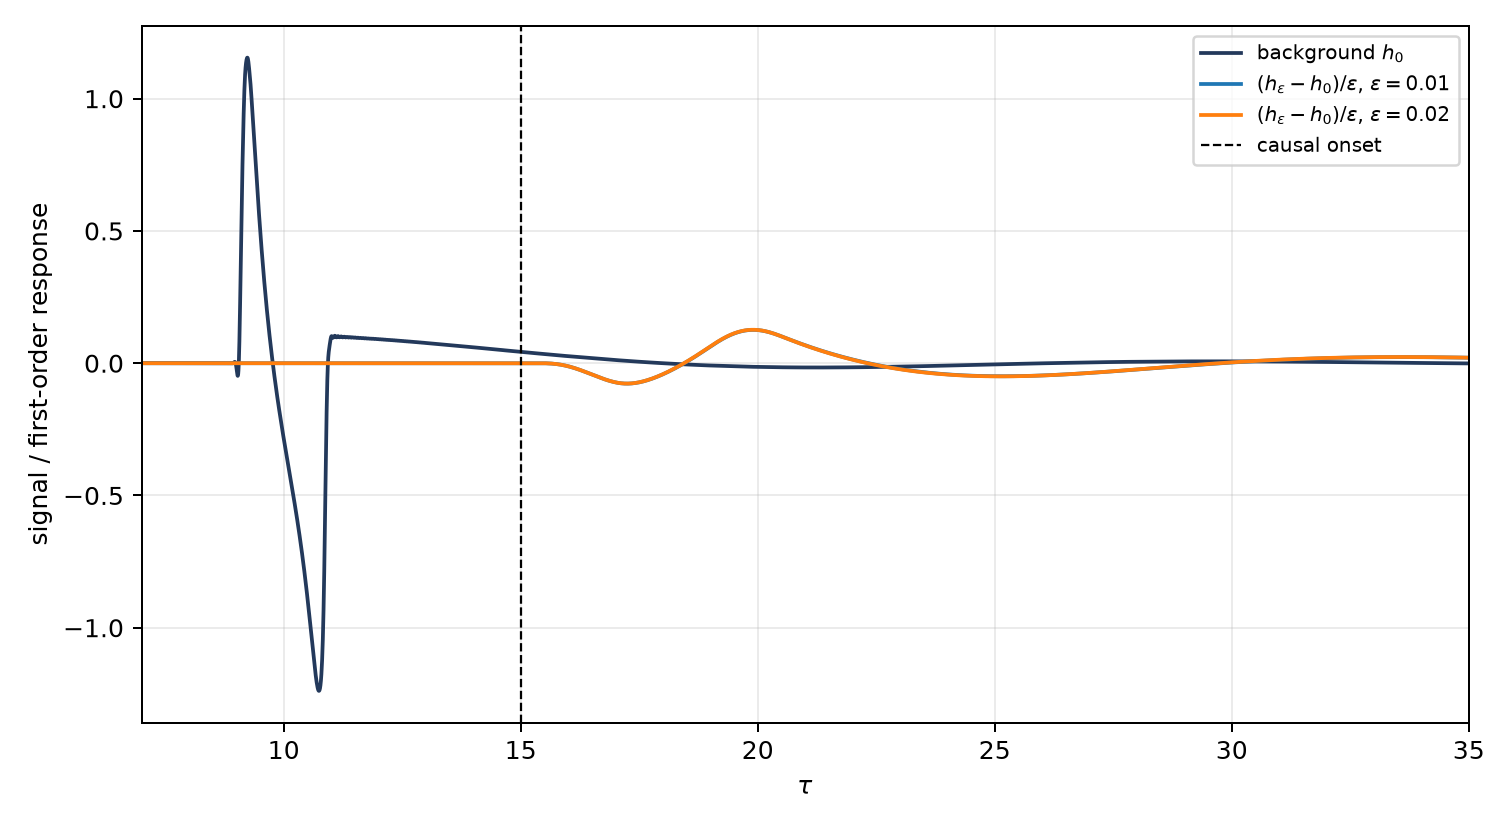
\includegraphics[width=0.95\textwidth]{waveform_check.png}
\caption{最细网格的背景信号及两组 $\ee$ 的归一化差波形；虚线为严格因果时刻 $t_*=15$。竖轴同时展示 $h_0$ 与 $(h_\ee-h_0)/\ee$，并非 (Q3a) 的积分误差。}
\end{figure}

\paragraph{证据边界与下一步。}
定理\ref{thm:causality}、\ref{thm:finite}、\ref{thm:spectrum}（在其注明的非退化与解析片条件下）、\ref{thm:log}以及判据\eqref{eq:criterion}是解析结论。上表仅为两网格数值复核。全时间一致的 (Q3c) 仍未闭合；应针对 $L\gg\log(1/\ee)$，尤其 $\omega\sim1/L$ 与 $\omega\sim\ee$，证明或证伪\eqref{eq:criterion}的实频积分一致界。若存在使该积分不按任何 $\ee^{2\alpha}$ 衰减的序列，就可构造 (Q3c) 反例；仅扩大有限时域网格而不控制边界和晚时低频峰不能给出该结论。本数学 mismatch 未使用探测器 PSD，也不构成实际可探测性断言；外部 bump 亦未被假定为 Einstein 方程的物质解。

\clearpage
\begin{thebibliography}{9}
\bibitem{ABW} L. Andersson, P. Blue and J. Wang, \emph{Morawetz estimate for linearized gravity in Schwarzschild}, \url{https://arxiv.org/abs/1708.06943}. 用于 Regge--Wheeler 局域衰减与全时间归一化存在性。
\bibitem{DSS} R. Donninger, W. Schlag and A. Soffer, \emph{On pointwise decay of linear waves on a Schwarzschild black hole background}, \url{https://arxiv.org/abs/0911.3179}. 用于零频尾巴与局域衰减背景。
\bibitem{Berti} E. Berti, V. Cardoso and A. O. Starinets, \emph{Quasinormal modes of black holes and black branes}, \url{https://arxiv.org/abs/0905.2975}. 用于标准 $l=2$ QNM 数值基准；本文没有独立重算该根。
\bibitem{Cheung} M. H.-Y. Cheung et al., \emph{Destabilizing the fundamental mode of black holes: The elephant and the flea}, \url{https://arxiv.org/abs/2111.05415}. 远 bump 谱迁移的相关背景。
\bibitem{Yang} Y. Yang et al., \emph{Spectral instability of black holes: Relating the frequency domain to the time domain}, \url{https://arxiv.org/abs/2407.20131}. 频域与早期波形对照的相关背景。
\bibitem{Kyutoku} K. Kyutoku, H. Motohashi and T. Tanaka, \emph{Quasinormal modes of Schwarzschild black holes on the real axis}, \url{https://arxiv.org/abs/2206.00671}. 实频相位与波形解释的相关背景。
\end{thebibliography}
\end{document}
